\documentclass{article}
\usepackage{amsmath} % for mathematical notation
\usepackage{tikz}
\begin{document}

\section*{17. Problema del vuelto}

\textit{En el problema del vuelto tenemos una cantidad ilimitada de monedas de distintos valores \( w_1, \ldots, w_k \) y queremos dar un vuelto \( v \) utilizando la menor cantidad de monedas posibles (ver Teórica 2). Por ejemplo, si los valores son \( w_1 = 1 \), \( w_2 = 5 \) y \( w_3 = 12 \), y el vuelto es \( v = 15 \), entonces el resultado es 3 ya que alcanza con dar 3 monedas de \( \$5 \). Modelar este problema como un problema de camino mínimo e indicar un algoritmo eficiente para resolverlo. El algoritmo sobre el modelo debe tener complejidad \( O(vk) \). Opcional: discutir cómo se relaciona este modelo con el algoritmo de programación dinámica correspondiente.}\\

Planteamos un grafo, donde tenemos \( v \) vértices, para cada valor entre 0 y 15, le sumamos nuestras \( k \) monedas y nos vinculamos con el vértice correspondiente. Si nos llegásemos a pasar de 15, no generamos ninguna conexión.

Por ejemplo, con la entrada dada en el enunciado:\\

Iniciamos en el 0, conectamos el vértice 0 a: 1, 5, 12, luego conectamos el 1 a: 2, 6, 13, y así sucesivamente.

Añadimos a cada arista un costo de 1. Luego usamos la función del ejercicio anterior para tomar el camino mínimo, con raíz en el 0 y final en el 15, ya que el grafo resultante es necesariamente un DAG. Nunca nos "restamos" monedas usadas, nuestro costo puede únicamente subir.

\begin{figure}[h]
\centering
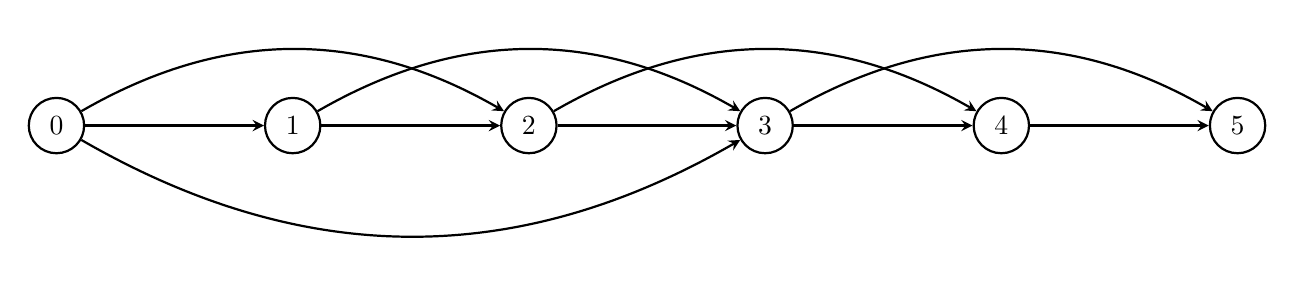
\begin{tikzpicture}[->,>=stealth,auto,node distance=3cm,thick]
    \tikzstyle{vertex}=[circle,draw,minimum size=20pt,inner sep=0pt]
    
    % Vertices
    \node[vertex] (0) at (0,0) {0};
    \node[vertex] (1) at (3,0) {1};
    \node[vertex] (2) at (6,0) {2};
    \node[vertex] (3) at (9,0) {3};
    \node[vertex] (4) at (12,0) {4};
    \node[vertex] (5) at (15,0) {5};
    
    % Edges
    \path
        (0) edge node {} (1)
        (0) edge[bend left] node {} (2)
        (0) edge[bend right] node {} (3)
        (1) edge node {} (2)
        (1) edge[bend left] node {} (3)
        (2) edge node {} (3)
        (2) edge[bend left] node {} (4)
        (3) edge node {} (4)
        (3) edge[bend left] node {} (5)
        (4) edge node {} (5)
        ;
\end{tikzpicture}
\caption{Grafo illustrando el problema del vuelto con monedas de \( 1, 2, \) y \( 3 \), con \( v = 5 \). Todas las aristas tienen coste 1}
\label{fig:coin_change_graph}
\end{figure}

\end{document}
